%%%%%%%%%%%%%%%%%%%%%%%%%%%%%%%%%%%%%%%%%%%%%%%%%%%%%%%%%%%%%%%%%%%%%%%%%%
\begin{frame}{Optimization Formulation}
The optimization of the films was formulated as finding the minimum mass of \iso[6]{Li} for a given detector material necessary to fulfill an interaction rate of \SI{2.5}{cps\per\nano\gram\iso[252]{Cf}} while maintaining a intrinsic gamma rejection ratio of \num{1.e-6}.
\end{frame}
%%%%%%%%%%%%%%%%%%%%%%%%%%%%%%%%%%%%%%%%%%%%%%%%%%%%%%%%%%%%%%%%%%%%%%%%%%
\subsection{Geometry Description}
\begin{frame}[fragile]{Gigantic Genome Geometries}
Genome BitString Representation
\begin{itemize}
  \item Divide the RPM8 width into even slices
  \item Compact representation of geometry, suitable for GA
  \item \verb+1+ - represents a detector assembly slice
  \item \verb+0+ - represents a moderator slice
  \item Example: \verb+001000+
  \begin{itemize}
    \item Each slice is \SI{2.12}{\centi\meter}
    \item Two slices of moderator, followed by one assembly slice followed by three additional slices of moderator
  \end{itemize}
\end{itemize}
\end{frame}
%%%%%%%%%%%%%%%%%%%%%%%%%%%%%%%%%%%%%%%%%%%%%%%%%%%%%%%%%%%%%%%%%%%%%%%%%%
\begin{frame}[fragile]{Computional Size}
\small
\begin{itemize}
  \item Each bit has two options, \verb+0+ or \verb+1+
  \item $2^n$ combinations for the search space - NP Hard!
  \item Each run takes about 1.72 minutes (16 cores)
\end{itemize}
\begin{table}
    \caption[Genome Bit String Geometries]{Bit String Simplified Geometetry Descriptions}
    \label{tab:BitStringGeo}
    \centering
    \tiny
    \begin{tabular}{ m{1.5cm} | m{1.5cm} m{1.5cm} m{1.5cm}  m{1.5cm}}
      Genome Length&Films Per Assembly&Slice Thickness&Light Guide Thickness&Possible Geomeries \\
      \hline
      \hline
      3&4&4.23&1.058&7 \\
      4&4&3.18&0.794&15 \\
      5&3&2.54&0.847&31 \\
      6&3&2.12&0.706&63 \\
      7&3&1.81&0.605&127 \\ 
      10&3&1.27&0.423&1023 \\
      13&2&0.98&0.488&8191 \\
      26&1&0.49&0.488&67108863 \\
    \end{tabular}
\end{table}
\end{frame}
%%%%%%%%%%%%%%%%%%%%%%%%%%%%%%%%%%%%%%%%%%%%%%%%%%%%%%%%%%%%%%%%%%%%%%%%%%
\begin{frame}
\begin{figure}
    \centering
    \begin{subfigure}[b]{0.45\textwidth}
        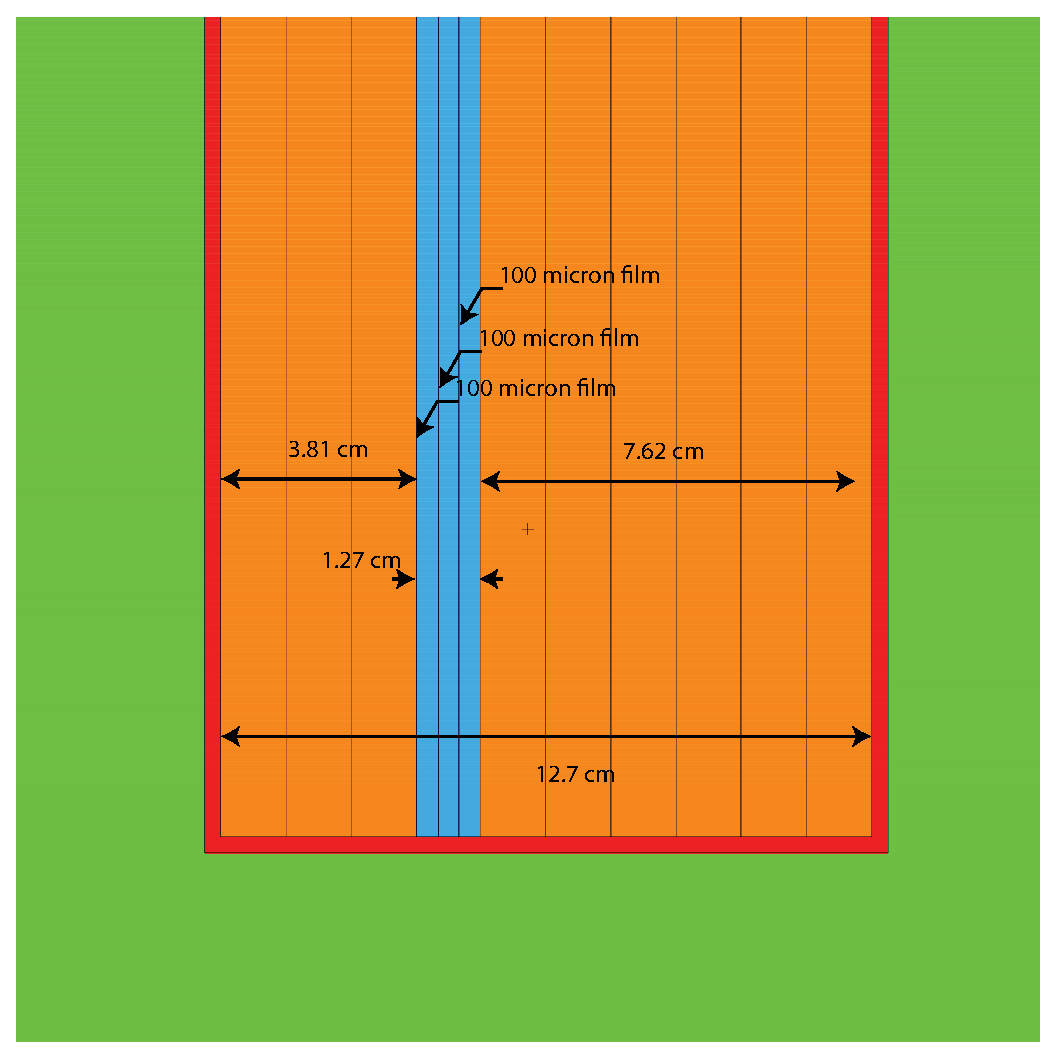
\includegraphics[width=\textwidth]{RPM8_Diagrams_MCNPXRender_10Opt}
    \end{subfigure}%
    ~
    \begin{subfigure}[b]{0.45\textwidth}
        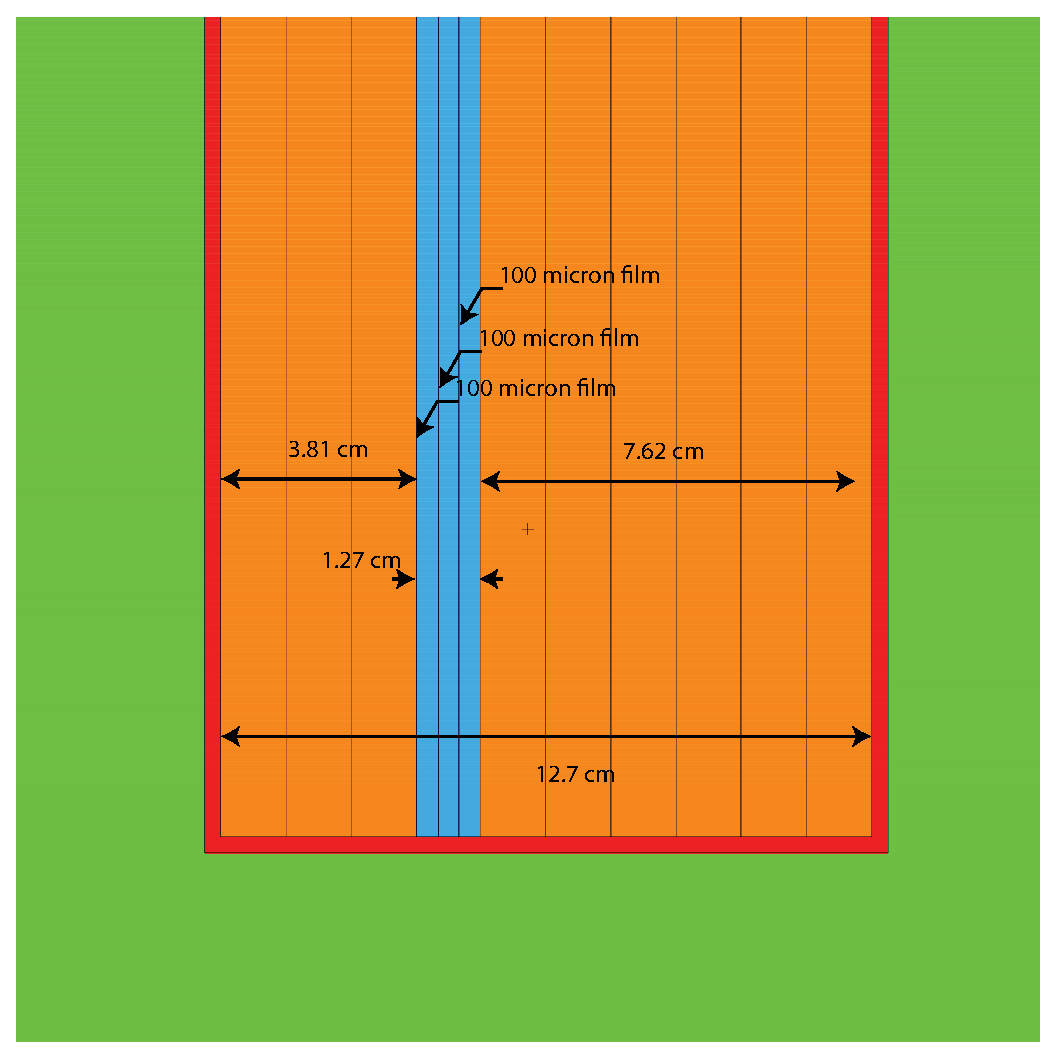
\includegraphics[width=\textwidth]{RPM8_Diagrams_MCNPXRender_26Opt}
    \end{subfigure}
    \caption{MCNPX rendering of layered geometry}
    \label{fig:MCNPXRendering}
\end{figure}
\end{frame}
%%%%%%%%%%%%%%%%%%%%%%%%%%%%%%%%%%%%%%%%%%%%%%%%%%%%%%%%%%%%%%%%%%%%%%%%%%
\subsection{Implemented Genetic Operators}
%%%%%%%%%%%%%%%%%%%%%%%%%%%%%%%%%%%%%%%%%%%%%%%%%%%%%%%%%%%%%%%%%%%%%%%%%%
\begin{frame}[fragile]{Mutation, Crossover and Selection}
  Operators from the PyEvolve toolkit
  \begin{itemize}
    \item Mutation - Flip Operator (2\%)
    \item Crossover - Single Point (90\%)
    \item Selection - Tournament Selection
  \end{itemize}
\end{frame}
%%%%%%%%%%%%%%%%%%%%%%%%%%%%%%%%%%%%%%%%%%%%%%%%%%%%%%%%%%%%%%%%%%%%%%%%%%
\begin{frame}{Fitness Function}
The fitness function was choosen to count rate per mass of \iso[6]{Li}, provided that the geometry meet the total count rate criteria.
If it failed to meet the count rate criteria a zero fitness was returned \eqref{eqn:FitnessFun}.
	\tiny
	\begin{align}
			\label{eqn:FitnessFun}
			f(\vec{x})
			= \begin{cases}
			0 & \text{if}~\text{countRate}(\vec{x}) \leq \SI{2.5}{cps\per\nano\gram\iso[252]{Cf}} \\
			\text{countRatePerMass}(\vec{x}) & \text{otherwise}
			\end{cases}
	\end{align}
\begin{columns}[onlytextwidth]
  \begin{column}{0.5\textwidth}
\small
	Computationally intensive to calculate the fitness function 
	\begin{itemize}
		\item Memoization with dictionaries
		\item Multithreading for items not in the dictionary
		\tiny
		\begin{itemize}
			\item This made it sensitive while running
			\item Future work would be to use the PyEvovle multithreading option
		\end{itemize}
	\end{itemize}
	\end{column}
	\begin{column}{0.4\textwidth}
    \begin{figure}
      \centering
      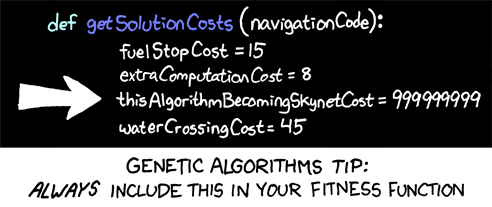
\includegraphics[width=\textwidth]{genetic_algorithms}
    \end{figure}
	\end{column}
\end{columns}
\end{frame}
%%%%%%%%%%%%%%%%%%%%%%%%%%%%%%%%%%%%%%%%%%%%%%%%%%%%%%%%%%%%%%%%%%%%%%%%%%
